\chapter{Fundamentals and Related Work\label{cha:chapter2}}

\section{Fundamentals in data unification\label{sec:unification}}

Electronic data processing underlies applied math and relies therefor on data of a certain, deterministic structure. In mathematics and computer science such rules of data representation are called canonical or normal form. Canonicalization is the discipline of transforming data of possible different forms of representation into a standardized form. An illustrative example of canonicalization is the representation of a boolean variable described in the XML schema type definition. By definition a boolean variable supports binary logic representation, meaning that some state or flag can either be true or false. The set of possible literals might contain: 1, 0, true and false. The XML schema type definition defines the canonical form of boolean as true and false, whereas 1 can be mapped to true and respectively 0 to false. Data in a normalized form can be transfered in any other form.
\\\\
The foundation of the idea of storing large data in a reusable format were captured by Edgar F. Codd in 1970 with his proposal for database normalization. The concept behind the proposal is to break the information down into entities with attributes and describe relations among them. A second and third version of database normalization followed and proposed a higher granularity. The technique of data normalization is state of the art in rational database systems. Such a system stores data in a table format, where rows correspond to entities and columns to their attributes. Considering the entities person and address as an example. The person entity has the attributes surname and name, the address entity the attributes street, zip code and city. In addition the person entity has a reference to the address entity, thus a an address can be related to a person. This relation is realized by a unique key. The system enforces the entity definition, i.e. its schema and the predefined data types, and the relationship constraints strictly. Relationship modeling plays also a fundamental role in other data base and data management systems but are often not enforced on system level.
\\\\
% https://db-engines.com/en/blog_post/23
In contrast to relational databases, normalization is not mandatory in non rational, also call no SQL databases. This kind of databases are mostly used for web applications and in the field of big data. The same applies to entity relationships as the core concept of no SQL databases aims for de-normalized data storage. Considering the person-address example from above, all attributes of a person entity are stored with it, including its address. No SQL databases exist with a schema-leas approach, meaning there is no predefinition of attributes and corresponding data types. This also enables changes of the schema over time in the cardinality of attributes as well as their type. In the person-address example this means that the address is a non mandatory field and the zip code can be stored as number or string. Document-oriented databases, key-value storages and graph databases are the three most common no SQL databases.  Limitations are only set by the user's definition and imagination. This flexibility enormously supports the initially claimed chaotic data storage, though it is often limited by schema definitions on domain level. 
\\\\
Schemas help to maintain a understandable structure of data and underly a certain format. They add determinism to data and make them less error prone. Schemas vary in their strictness, also formats allow different levels of precision. CSV, JSON and XML are the most commonly used formats for data interchange, whereas JSON holds a distinguished position nowadays. From a top down view on entity level they define the set of attributes an information entity has. In addition it is possible to define whether a field is mandatory or not. Furthermore a schema can be designed such that it enforces entity relations. On attribute level the most common specification is the data type, whereas the information if a field can be unset, i.e. nullable, can be provided too. Data types are usually not unique through different schema formats, but mappings usually exist. For a higher quality of data the individual type of an attribute can be restricted through ranges or enumerations, e.g. the value of field score can only accept integers from 1 to 5. Furthermore it is to distinguish between externally defined and self-contained schemas. External definition or external enforcement is the approach that drives rational databases and schema-full data storages. Is the schema woven with the actual data, one can speak about self-contained schemas. Schema-less storages benefit from self-contained schemas. Using such, data integrity it is for the application level to maintain.
\\\\
The canonical form standardizes data representation, whereas normalization and schema definition add some additional information to it. A predefined cardinality of attributes as well as the respective types and value ranges can be considered as meta-data and make the data therefor more understandable by human as well as by machines. 

\section{Data storage technologies and data formats\label{sec:storage}}

In data driven applications the data are commonly fetched from a source. Sources in this circumstances are wide-ranging. A few to mention here are:
\begin{itemize}
  \item Purely file based, e.g. CSV files
  \item Database systems (rational database management systems, key-value stores, document-oriented)
  \item REST interfaces
  \item Web sockets
  \item Message queues\\
\end{itemize}

\noindent\textbf{Purely file based} have almost no restrictions regarding the information format. The format is often defined on domain level. Human readable formats like CSV, JSON, XML or custom formats are some of the most common data structures. Additionally binary formats exists but are more often used in closed systems.
\\\\
\textbf{Database systems} provide more boundaries when it comes to the data format. Database management system can be divided in schema-oriented and schema-less systems. The former, by definition, enforces a certain schema for individual information entities. In rational database systems most often a table format is chosen, but also in key-value stores the format of the value might be enforced by the system. Schema-less systems, also often document-oriented, bring more flexibility. The format, in many cases JSON, has to be defined per type of information entities. The actual schema, i.e. definition of attributes, is not enforced in such systems.
\\\\
\textbf{REST interfaces} deliver data in most cases in human readable format. Some exception exist that expose binary information. The so called media type, also MIME type or content type, is officially standardized by the Internet Assigned Numbers Authority (IANA). Dedicated content delivery APIs mostly utilize pain text, JSON or XML. For memory reduction zipped data are shipped. 
\\\\
\textbf{Web sockets} are originally designed for the communication between browsers and web servers and lower network layer, TCP, as REST interfaces for data exchange. Projects exists where web sockets are used for data transfer and enables a streaming unlike REST, which works on a batch basis. Regarding data formats, web sockets apply similarly loose restrictions regarding formats as file based data sources does.
\\\\
\textbf{Message queues} are old techniques but embrace over the last years enormously. The trends shifts towards data streaming and directly process them rather to store data over the long-term. Often used for connecting systems, message queues do most often not enforce a specific data formats also similar to file based sources.

\section{State analysis of heterogeneous data storage\label{sec:stateanalysis}}

\begin{figure}[htb]
  \centering
  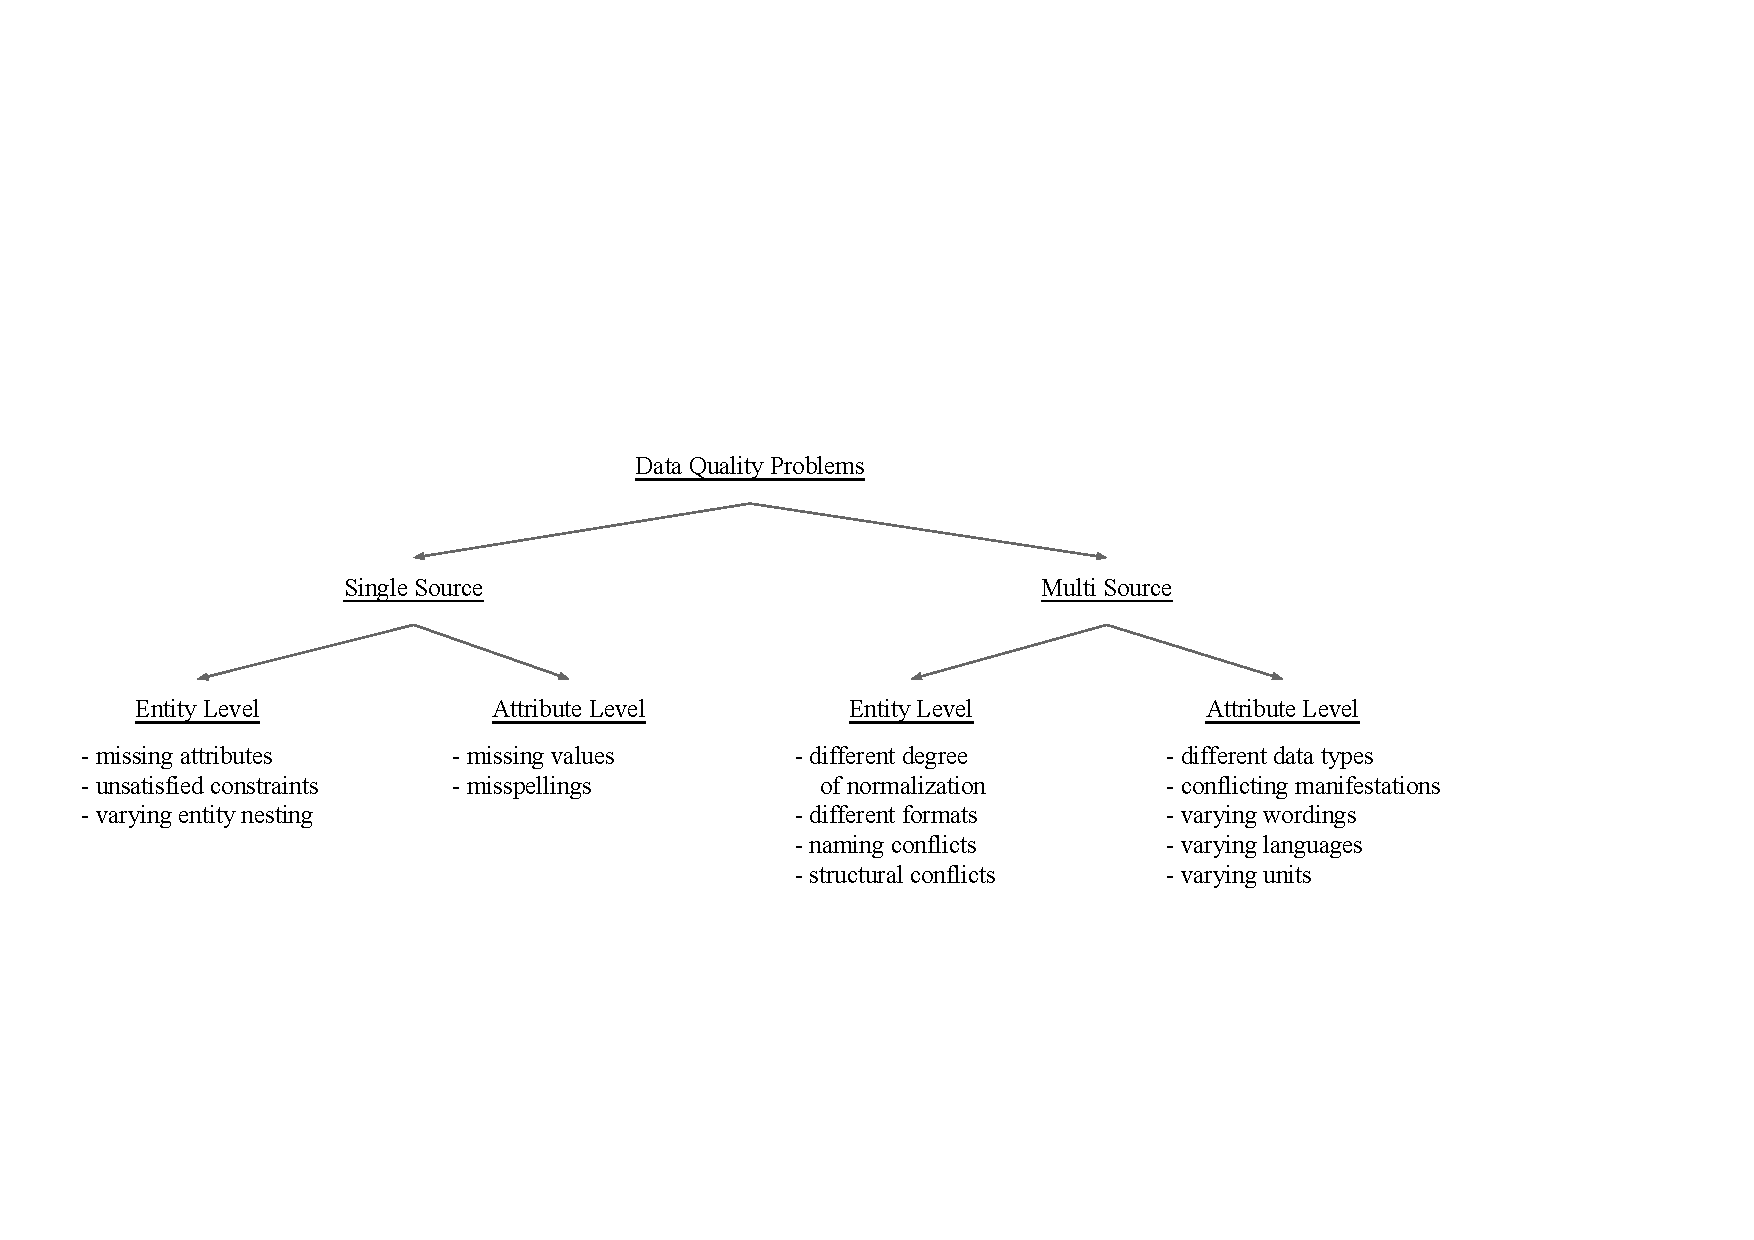
\includegraphics[width=0.9\textwidth]{quality-problems.pdf}\\
  \caption{Categorization of data quality problems}\label{fig:qualityproblems}
\end{figure}

In this section digitally available data are analyzed with respect to their quality as well as considering their source. Figure \ref{fig:qualityproblems} illustrates a categorization of the data quality issues into four sub problems. The breakdown shows that the devision correlates with the above stated classification of data storage principles. Therefor a general distinction between single and multi source problems is possible. In both categories a distinction on entity level can be made. 

\subsection{Single source problems}

Single source problems consider malformed data within one storage system. A single source normally is maintained by a single instance and can be considered as less messy as a multi source environment. Nevertheless even such system contain malformed data which can not be directly used for analysis.

Schema-less systems can be considered as more error prone than systems enforcing a schema. In the former unsatisfied constraints occur whereas in the latter additionally missing attributes and varying entity nesting arise. Those problems are mostly schema related and occur due to poorly designed schemas, technical depts or negligence of specifications. Attribute level specific issues can only partly covered by schema definitions. For instance, missing values are coverable but not spelling errors. Table \ref{tab:singlesource} outlines examples conflicts occurring on data unification. 

Missing attributes or missing values no not necessarily indicate malformed data. Information entities exist where the absence of data actually provides insights. Declaration on specification level increases the interpretability and analyzability of latent information accordingly. Broken constrains reflect inconsistent and missing data. Compare row one of table \ref{tab:singlesource}.

The second row of table \ref{tab:singlesource} shows an person entity referring to a non-existing address. Data are not usable under original condition and has to be re-interpreted. In document-oriented databases can be nested within sub-entities but basically providing equal information. On unification such data structures conflict and require exceptional treatment. 

% TODO nesting

Another potential conflict arises when it comes to standardizing data are missing values. An example is provided in row four of table \ref{tab:singlesource}. Unset values can be interpreted in two fashions. It can mean on one hand, that the value for that attribute is not captured, i.e. the value exists but is not present, on the other hand it can imply that it can not be captured, i.e. the attribute is not available for that entity. Whereas the former is the correct interpretation in terms of data management, it is widely abused in the sens of the latter definition. The interpretation is up to the maintainer of the data source. A further problem in both cases are missing values on mandatory fields in respect of future data processing.

Misspelling are faulty data from manual entry. The problem of such when it comes to heterogeneous data aggregation is the same problematic as in homogeneous environment and therefor plays a very critical role for example if information are displayed to end users.  

\begin{table}[htb]
\centering
\resizebox{\textwidth}{!}{
\begin{tabular}[t]{|l|l|}
\hline
Problem & Example \\
\hline
\hline
Missing & Person\textsubscript{1}(name="Fritz", age="23", city="Berlin") \\
attribute & Person\textsubscript{2}(name="Eva", city="Berlin") \\
\hline
Unsatisfied & Person\textsubscript{1}(name="John", addressId="1") \\
constraints & \\
\hline
Varying entity & Person\textsubscript{1}(name="Fritz", street="Spanische Straße 17", city="Berlin") \\
nesting & Person\textsubscript{2}(name"Eva", address=Adress(street="Baumallee 34", city="Berlin")) \\
\hline
Missing & Person\textsubscript{1}(name="Fritz", age="23", city="Berlin") \\
values & Person\textsubscript{2}(name="Eva", age="", city="Berlin") \\
\hline
\end{tabular}
}
\caption{Examples of single source problems}
\label{tab:singlesource}
\end{table}

\subsection{Multi source problems}
All problems from a single source environment can be transfered to a multi source environment. Additionally the absence of commonly valid schema definitions fosters problems when it comes to unification of data and information among various sources. The sub categorization of multi source problems goes along with the sub categorization of single source problems. On entity level issues due to different degrees of normalization, different formats, naming conflicts or structural conflicts are possible discrepancies. On attribute level different data types, conflicting manifestations, languages and units prevent a simple solution to data unification.

One big challenge in data source fusion is a different degree of normalization or granularity of data. Highly depending on the use case the data are collected for, attributes are broken down into different abstraction levels. For that reason one attribute in one source can correspond to two or more attributes in a second source. Depending on the storage technology used the same information are de-normalize, i.e. one entity captures all information, or completely normalized, i.e. split up into two entities. Row one in Table \ref{tab:multisource} shows three information entities that basically contain the same data but in different forms of normalization. Normalization of fields requires in some cases significant domain knowledge. 

Section \ref{sec:unification} provided an overview of different data formats. Every one has its on semantic and characteristics. A straight forward aggregation among two data formats is barely possible. For instance, comparing the JSON format with CSV shows, the first supports nesting of entities the other not. XML and JSON on the other hand support both nesting but distinguish in incompatible data types, as JONS for instance can not represent long integers, whereas XML supports this data type.

A well known problem is the parsing of addresses, especially street names and house numbers. From an automation point of view it is impossible to perform accurate splitting of that fields. This is a crucial point if the desired output format requires a higher degree of normalization than some of the underlying sources can provide. Row two in table \ref{tab:multisource} shows an example of different schema definition in terms of attribute naming. Fields containing equal information are annotated by a different name. In this example the fields \textit{city} and \textit{town} hold the home town of the person captured. This heterogeneity can also be the source of usage of different languages, e.g. American English and British English. 

As already explained in \ref{sec:unification} storage formats support different data types. Not only technical restrictions but also domain specific restrictions require a different choice of data type for the same type of information. As an example we can consider the ZIP code. For some countries it is sufficient to use an integer type for others its is mandatory to store the postal code as string, as non-numeric characters are contained. Compare row three in table \ref{tab:multisource}. 

Enums provide a predefined set of manifestations for a certain attribute. Usually designed to avoid messy data enums can in fact cause discrepancies during data unification. This problem is similar to the attribute naming problem mentioned above: Different manifestations stand for the same information value. The problem becomes more severe if a direct mapping among sources into one distinct target format is not possible. In system A a entity can accept n different states, whereas in system B m different states are possible. See row four in table \ref{tab:multisource} for comparison.

Similar to differing manifestations is the problem of different units. Two example entities can be seen in row 5 of table \ref{tab:multisource}. The problem is of a higher complexity as quantities are also affected. Especially for mathematical data analysis a common system of units is essential. Combining data from multiple sources must consider such inequalities otherwise aggregations results are faulty.

All multi source problems can be applied as outlined here to schema-less data storages. 

\begin{table}[htb]
\centering
\resizebox{\textwidth}{!}{
\begin{tabular}[t]{|l|l|}
\hline
Problem & Example \\
\hline
\hline
Different degree & Person\textsubscript{1}(name="Fritz", address="Spanische Straße 17, Berlin") \\
of normalization & Person\textsubscript{2}(name="Eva", street="Baumstr.", no="34", city="Berlin") \\
 & Person\textsubscript{3}(name="John", adrId="1"), \\
 & Address(adrId="1", street="Weg", no="2", city="Berlin") \\
\hline
Naming & Person\textsubscript{1}(name="Fritz", city="Berlin") \\
conflict & Person\textsubscript{2}(name="Eva", town="Berlin") \\
\hline
Different & Address\textsubscript{1}(zip="24821", city="Berlin") \\
data types & Address\textsubscript{2}(zip=24821, city="Berlin") \\
\hline
Different & Product\textsubscript{1}(name="apple", status="new") \\
Manifestations & Product\textsubscript{2}(name="apple", status="created") \\
\hline
Different & Product\textsubscript{1}(name="apple", amount="1", unit="ea") \\
Units & Product\textsubscript{2}(name="apple", amount="1", unit="kg") \\
\hline
\end{tabular}
}
\caption{Examples of multi source problems}
\label{tab:multisource}
\end{table}

\section{Assessment of problems for feature extraction\label{sec:problemassesment}}

Based on the previous section an assessment of the revealed problems. Indicator as their severity and complexity are considered and finally used to identify concrete issues handed within this work. 
\\\\
Unsatisfied constraints are a general problem in no SQL systems and need to be enforced on application level. Broken constraints are therefor not considered as a major problem of homogenization of data sources. The same applies to misspelling errors. This type of error is required to run through spell checking software and needs extended manual quality checks for appropriate correction. 
\\\\
The main focus in this work will be on unifying data for automated feature extraction that underly the problems of structural issues. Automation technologies an methods need to be identified and applied reasonable. This covers the sub problem like missing attributes, naming issues and varying entity nesting.
\\\\
As second aspect differing levels of normalization are in the focus of this thesis. This is due to the fact, that preliminary information from modern storage systems, e.g. schema-less databases are to be analyzed as they make up a significant amount of latest data in web applications.
\\\\
As third an last main focus problems towards different manifestations are chosen. Especially categories and labels for data are very important in modern machine learning approaches. Features extracted from this kind of information provide value in applications like predictions and recommendations.

\section{Related Literature and Technologies \label{sec:tech}}

% http://dl.acm.org/citation.cfm?id=1541883&CFID=963228341&CFTOKEN=32205688

This section describes relevant technologies, starting with X followed by Y, concluding with Z.

* ETL
